\chapter{ Cl\^{o}ture du projet }

\section{Introduction}

La phase cl\^{o}ture ou de fermeture est la derni\`{e}re phase dans le cycle de d\'{e}veloppement d'un
logiciel avec Scrum. Cette phase est souvent appel\'{e} sprint de stabilisation. Les t\^{a}ches
effectu\'{e}es pendant cette phase pr\'{e}d\'{e}finies, et ils d\'{e}pendent fortement du type de projet.
Pour notre projet, ce chapitre sera consacr\'{e} pour la pr\'{e}sentation des langages et outils de
programmation utilis\'{e}s pour la r\'{e}alisation de nos deux applications.



\section{Impl\'{e}mentation et structure}
Enfin nous d\'{e}crivons les \'{e}tapes globales suivies lors de la r\'{e}alisation de ce projet.
Les \'{e}tapes \'{e}taient :
\bigskip


\textbullet{}  Cr\'{e}er le site web statique (front -end)  \newline
\textbullet{} Cr\'{e}er une application express js  \newline
\textbullet{}  Cr\'{e}ation du base de donn\'{e}es et liaison des donn\'{e}es par le driver node js  de mysql \newline
\textbullet{}Cr\'{e}er un rest api \`{a} l'aide de express js  \newline
\textbullet{}Int\'{e}gration de front-end avec le back-end  \newline
\textbullet{}Ajout des modules suppl\'{e}mentaire (Authentification avec jwt et gestion des roles utilisateur et administrateur)  \newline
\textbullet{}  H\'{e}bergement en ligne de la base de donn\'{e}es \newline
\textbullet{} H\'{e}bergement en ligne de l'application web  \newline




\section{Application en ligne}
Vous pouvez trouvez l'application sur le lien [13].


  Pour acc\'{e}der en tant qu'administrateur veuiilez utiliser:

  \begin{itemize}
    \item {\textbf{ Pseudo:}admin}
    \item {\textbf{ Password:}0000}
  \end{itemize}


  Pour acc\'{e}der en tant que membre 'Wael Chorfan' par exemple veuillez utiliser:

  \begin{itemize}
    \item {\textbf{ Pseudo:}WC}
    \item {\textbf{ Password:}0001}
  \end{itemize}

 \newpage



 \section{ Architecture 3 tiers}

Notre projet est caract\'{e}ris\'{e} par son architecture 3 tiers qui inclus un mod\`{e}le MVC (Mod\`{e}le
Vue Contr\^{o}leur)

\begin{itemize}
  \item { Machine: acc\`{e}s et mise \`{a} jour des donn\'{e}es.}
  \item {Back-End express Server : contient l'application.}
  \item {MySql: gestion de donn\'{e}es et mise \`{a} jour.}
  
\end{itemize}



\section{Environnement de d\'{e}veloppement}

  \subsection{Environnement mat\'{e}riel }

  Pour la r\'{e}alisation du projet, nous avons utilis\'{e}un ordinateur
  portable pour le d\'{e}veloppement ayant les caract\'{e}ristiques suivantes :

\begin{itemize}
  \item {  Mod\`{e}le : Asus XJ550 }
  \item {Processeur : i7 2.6GHz }
  \item {Disque Dur : 1To }
  \item { Syst\`{e}mes d'exploitation : Windows 7  }
  \item {M\'{e}moire : 8Go}

\end{itemize}





  \subsection{Environnement logiciel}


L'environnement logiciel utilis\'{e} pour r\'{e}aliser notre projet est comme suit : \newline

\begin{itemize}



\item {  \textbf{MySQL} }


C'est un syst\`{e}me de gestion de bases de données relationnelles. Il est distribu\'{e}
sous une double licence GPL et propri\'{e}taire. Il fait partie des logiciels de gestion
de base de donn\'{e}es les plus utilis\'{e}s au monde.

Nous avons uutilis\'{e} wamp (phpmyadmin)[5]  en local et remote mysql pour l'h\'{e}b\'{e}rgement en ligne[6]. \newline



\FloatBarrier
\begin{figure}[H]
\center

\includegraphics[width=6cm,height=4cm]{./figures/teklogos/phpmyadmin.png}
\caption{phpmyadmin.}
\end{figure}
\FloatBarrier

\FloatBarrier
\begin{figure}[H]
\center

\includegraphics[width=6cm,height=4cm]{./figures/teklogos/wamp.png}
\caption{Wamp.}
\end{figure}
\FloatBarrier

\item {  \textbf{Visual Studio Code} } [1]

est un \'{e}diteur de code extensible d\'{e}velopp\'{e} par Microsoft pour Windows,
Linux et OS X.
Nous avons utilis\'{e} visuel code pour \'{e}crire le code de l'application. \newline


\FloatBarrier
\begin{figure}[H]
\center

\includegraphics[width=6cm,height=4cm]{./figures/teklogos/vscode.png}
\caption{Visual Studio Code.}
\end{figure}
\FloatBarrier
\item {  \textbf{StarUML} } [14]

StarUML est un logiciel de mod\'{e}lisation UML, c\'{e}d\'{e} comme open source par son \'{e}diteur, \`{a} la
fin de son exploitation commerciale, sous une licence modifi\'{e}e de GNU GPL, Nous avons fait
les diagrammes avec cette technologie.


\FloatBarrier
\begin{figure}[H]
\center

\includegraphics[width=6cm,height=4cm]{./figures/teklogos/staruml.png}
\caption{Staruml.}
\end{figure}
\FloatBarrier


\section{Outils et technologies }

\item {  \textbf{Node js} } [2]

Framework javascript ,nous l'avons utilis\'{e} pour cr\'{e}er le serveur web .
Il offre la rapidit\'{e} de ,la performance etla modularit\'{e}.\newline

\FloatBarrier
\begin{figure}[H]
\center

\includegraphics[width=6cm,height=4cm]{./figures/teklogos/node.png}
\caption{Node js.}
\end{figure}
\FloatBarrier

\item {  \textbf{ Express js} } [3]



 C'est un framework pour construire des
 applications web bas\'{e}es sur Node js .
 Il  sert \`{a} cre\'{e}r l'application ,il est en
relation avec la base de donn\'{e}es par le biais de driver mysql et en relation
avec les modules web par le moteur de vues EJS.\newline


\FloatBarrier
\begin{figure}[H]
\center

\includegraphics[width=6cm,height=4cm]{./figures/teklogos/express.png}
\caption{Express js.}
\end{figure}
\FloatBarrier



\item {  \textbf{ Postman:} } [16]


Est le seul environnement de d\'{e}veloppement d'API complet utilis\'{e} par plus de 7 millions
de d\'{e}veloppeurs et 200 000 entreprises dans le monde
cela rend le d\'{e}veloppement d'API plus rapide,
 plus facile et plus performant.

\FloatBarrier
\begin{figure}[H]
\center

\includegraphics[width=6cm,height=4cm]{./figures/teklogos/postman.png}
\caption{Postman.}
\end{figure}
\FloatBarrier

\item {  \textbf{ Vue js:} } [11]

Framework javascript front-end utilis\'{e} pour la programmation et la
manipulation des actions,entr\'{e}es et sorties des diff\'{e}rents modules . \newline
\FloatBarrier
\begin{figure}[H]
\center

\includegraphics[width=6cm,height=4cm]{./figures/teklogos/vue.png}
\caption{Vue js.}
\end{figure}
\FloatBarrier

\item {  \textbf{ Mysql js:} } [12]


Langage de la base de donn\'{e}es relationnelle utilis\'{e}e.
e.EJS moteur de vue d'express js , ce type permet l'intercommunication entre
les modules web et le serveur . \newline
\FloatBarrier
\begin{figure}[H]
\center

\includegraphics[width=6cm,height=4cm]{./figures/teklogos/mysql.png}
\caption{MySQL.}
\end{figure}
\FloatBarrier

\item {  \textbf{ EJS:} } [10]


moteur de vue d'express js , ce type permet l'intercommunication entre
les modules web et le serveur . \newline

\begin{figure}[H]
\center
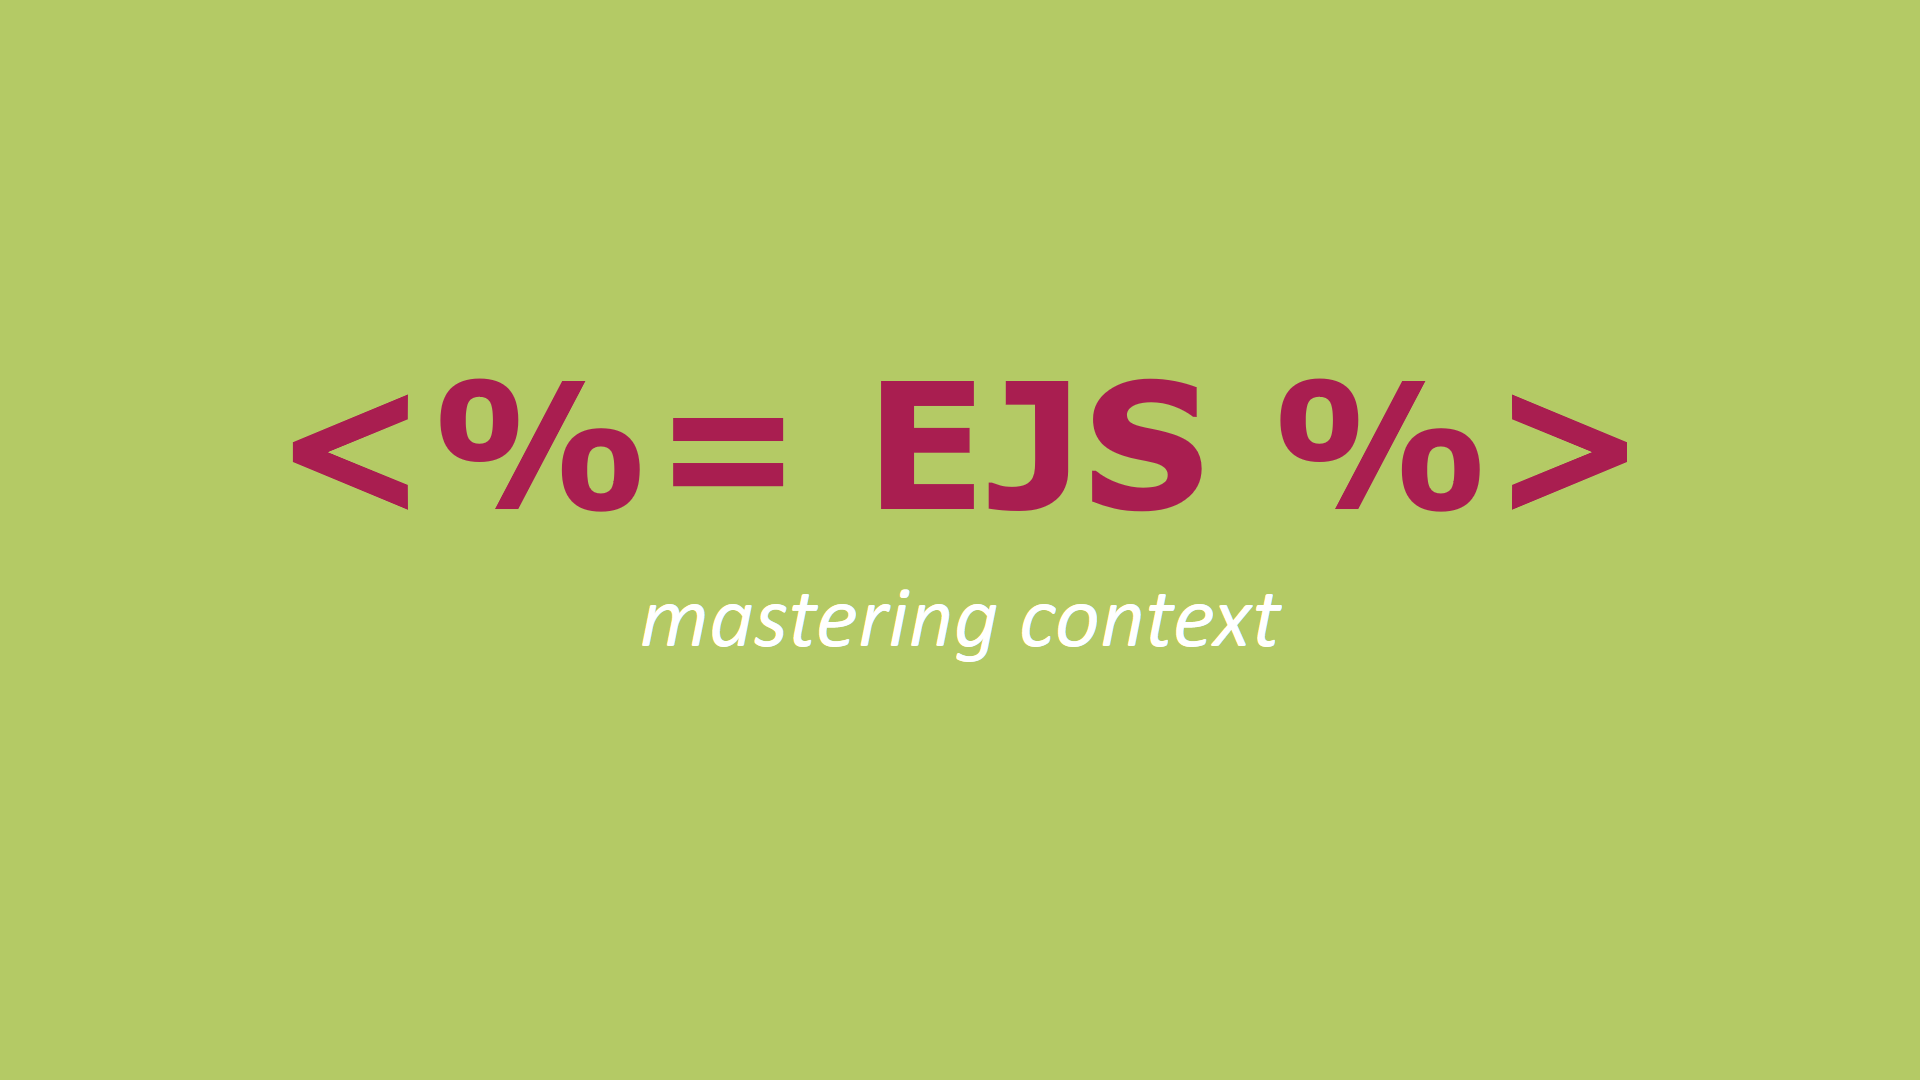
\includegraphics[width=6cm,height=4cm]{./figures/teklogos/ejs.png}
\caption{EJS.}
\end{figure}


\item {  \textbf{ Talend:} } [17]


 Est un éditeur de logiciel basé sur le langage JAVA spécialisé dans l'intégration de données.


\begin{figure}[H]
\center

\includegraphics[width=6cm,height=4cm]{./figures/teklogos/talend.png}
\caption{Talend.}
\end{figure}


\item {  \textbf{ Highcharts:} } [15]


L'outil de \guillemotleft{} reporting \guillemotright{} sur les pages web.


\begin{figure}[H]
\center

\includegraphics[width=6cm,height=4cm]{./figures/teklogos/highcharts.png}
\caption{Highcharts.}
\end{figure}


\end{itemize}


\section{Conclusion}

Dans ce chapitre, nous avons présenté l’architecture de notre système ainsi que
l’environnement matériel et logiciel nécessaire pour notre travail.


















